\documentclass[preprint,12pt]{elsarticle}

% =========================================================
% Packages
% =========================================================
\usepackage{amsmath,amsfonts,amssymb,bm}
\usepackage{amsthm}
\usepackage{graphicx}
\usepackage{booktabs,array,multirow}
\usepackage{url}
\usepackage{textcomp}
\usepackage{algorithm}
\usepackage{algorithmic}
\usepackage[protrusion=true,expansion=false]{microtype}
\usepackage[hidelinks]{hyperref}
\usepackage{placeins}
\usepackage{float}
\usepackage{tabularx}
\usepackage{ragged2e}
\usepackage{longtable}
% Numbered citations compressed as [1--3]
\biboptions{sort&compress}

% =========================================================
% Theorem environments
% =========================================================
\newtheorem{theorem}{Theorem}[section]
\newtheorem{corollary}[theorem]{Corollary}
\newtheorem{proposition}[theorem]{Proposition}
\newtheorem{assumption}[theorem]{Assumption}
\newtheorem{remark}[theorem]{Remark}

\hyphenation{
	op-tical
	net-works
	semi-conduc-tor
	PAC-Bayesian
	Takagi-Sugeno
}

% =========================================================
% Journal
% =========================================================
\journal{Engineering Applications of Artificial Intelligence}

\begin{document}
	
	% =========================================================
	% Front matter
	% =========================================================
	\begin{frontmatter}
		
		\title{
			An Auditable Complexity-Aware PAC-Bayesian Framework for
			Linear and Takagi--Sugeno Time-Series Forecasting under
			Temporal Dependence
		}
		
	
		
	\begin{abstract}
		PAC-Bayesian certificates can provide useful risk guarantees for
		time-series forecasting, but their practical value depends on how the
		prior, loss, and model-selection choices are constructed. This paper
		presents an auditable framework for linear and first-order
		Takagi--Sugeno (TSK) forecasting under overlapping and potentially
		nonstationary observations. The method uses a chronological data split
		to construct valid priors and an explicit hierarchical code to account
		for model family, lag, regularization, radius, rule count, localization,
		and prior scale. The resulting certificate applies to clipped Gibbs risk
		and the clipped Bayesian model average, while deterministic forecasts
		use it only as a screening criterion.
		
		Experiments on 30 synthetic series show that reducing complete TSK rule
		blocks lowers parameter dimension, Gaussian KL divergence, and the
		certificate relative to a dense 12-rule model. However, a sensitivity
		analysis over several fixed rule counts shows that much of this gain is
		due to using fewer rules, and radius control does not consistently
		outperform small fixed-$K$ models. Multi-rule examples illustrate the
		learned local structures. In the energy studies, a stricter frozen gate
		improves performance over a seasonal-naive fallback on four PJM regions,
		although post-hoc SARIMA and ETS models remain competitive. Overall, the
		results support auditable complexity control and conservative model
		screening rather than a general claim of TSK superiority.
	\end{abstract}
	
	
		\begin{keyword}
			PAC-Bayesian learning \sep
			Takagi--Sugeno fuzzy systems \sep
			time-series forecasting \sep
			martingales \sep
			temporal dependence \sep
			structural sparsity \sep
			risk certificates
		\end{keyword}
		
	\end{frontmatter}
	
	% =========================================================
	% Main manuscript
	% =========================================================
	\section{Introduction}
\label{sec:introduction}
Reliable energy load forecasting is a cornerstone of modern power-grid operation, 
directly affecting unit commitment, reserve scheduling, and market clearing 
decisions. In deregulated markets such as the PJM Interconnection, day-ahead and 
real-time forecasts must remain accurate across diverse regional load profiles that 
exhibit strong seasonality, overlapping temporal dependence, and occasional 
structural shifts driven by weather extremes or policy changes. Conventional 
workflows select predictors by validation error and assess them on a held-out 
horizon. While this measures empirical forecasting performance, it does not by 
itself quantify the conditional risk of a data-dependent model when lagged examples 
overlap, the observations are temporally dependent, and the underlying process may 
change over time.
Takagi\-\-Sugeno (TSK) fuzzy systems represent an attractive middle ground for this 
setting: they capture nonlinear dynamics through convex combinations of local 
affine rules, offer interpretable antecedent--consequent structures, and can be 
trained efficiently when the rule base is fixed. Their operational behaviour, 
however, depends on several jointly selected structural and numerical choices---lag 
order, antecedent geometry, number of rules, and regularization of the consequent 
parameters---that affect accuracy, interpretability, and effective statistical 
complexity. In many forecasting studies, the rule count and consequent dimension 
are treated as implementation details rather than explicit components of a 
generalization audit. Consequently, a deployed TSK model may carry uncharged 
complexity that undermines its reliability when the process shifts.
PAC-Bayesian analysis provides a natural language for relating empirical loss to a 
prior--posterior complexity term, yet its practical value in sequential forecasting 
depends on how the prior, the loss, and the model-selection choices are 
constructed. A certificate can be misleading if the prior is localized with 
certification observations, squared loss is treated as bounded without 
justification, or lag, regularization, radius, and rule-count choices are selected 
without paying their complexity cost. Moreover, a non-vacuous certificate need not 
identify the predictor with the lowest raw test RMSE or the best operational cost; 
it is, instead, a conservative screening statistic that can be integrated into a 
broader expert-system deployment rule.
This study develops an auditable expert-system framework for linear and first-order 
TSK load forecasting under overlapping and potentially nonstationary windows. The 
time-uniform supermartingale argument used in the analysis is established in the 
PAC-Bayes literature and is not presented as a new concentration theorem. The 
methodological contribution lies in the chronological construction of the candidate 
priors, explicit hierarchical charging of the complete model index, analytic 
evaluation of a Gaussian empirical-risk upper bound, separation of structural 
sparsity from activation sparsity, and integration of the certificate into a frozen 
model-selection and abstention protocol that mimics operational decision-making.
The central claim is deliberately limited. We do not introduce a new fuzzy 
clustering algorithm, prove that radius-based rule construction dominates all fixed 
rule bases, or show that TSK models universally outperform linear and seasonal 
predictors. Instead, we ask whether complete removal of rule blocks makes TSK 
complexity auditable and whether a valid certificate can serve as one conservative 
screening component inside a broader deployment rule for energy forecasting.
The contributions of this expert-system framework are as follows.
\begin{itemize}
	\item We define a chronological candidate family with complete structural
	index $M=(F,p,\gamma,r,K)$, where $F$ denotes the model family, $p$ the
	lag, $\gamma$ the ridge penalty, $r$ an optional radius, and $K$ the realized
	rule count. Scaling, antecedent geometry, prior means, and prior variances are constructed only from the initial segment, ensuring auditability.
	\item We provide a computable bounded-loss specialization of the established	time-uniform supermartingale PAC-Bayes framework \cite{chugg2023unified}. The contribution is the measurable linear/TSK specialization, augmented hierarchical prior, analytic empirical-risk upper bound, and audited	implementation suitable for operational screening.
	\item We distinguish structural rule-count reduction from sparse activation.
	A synthetic development study compares ridge, fixed-$K$ TSK, radius-controlled
	all-active TSK, and radius-controlled Top-3 TSK. A subsequent sensitivity
	analysis over $K \in \{2,3,4,6,8,12\}$ separates the effect of reducing rule
	count from any additional benefit of radius construction.
	\item We expose actual posterior-center fuzzy rules from a multi-rule SETAR
	model and from the Tetouan development model. These examples support
	inspection of the learned local structures without treating them as physical
	truth or as directly certified deterministic predictors.
	\item We report a negative Tetouan development gate and an internally locked
	PJM holdout evaluation. Secondary SARIMA, exponential-smoothing, and deep
	learning benchmarks are explicitly labeled post hoc because they were designed
	after the PJM outcomes were opened and do not modify the frozen gate or its
	original claim.
\end{itemize}

The evidence supports an integration claim for operational expert-system deployment
rather than a fuzzy-model superiority claim. Structural rule reduction substantially
lowers dimension, KL divergence, and certificate value relative to an unnecessarily
dense 12-rule TSK model. Small fixed rule bases can, however, match or tighten the
radius-controlled certificate, and ridge remains the easiest family to certify on
average. The independent PJM energy decisions mostly select linear predictors,
while the secondary statistical and deep-learning baselines show that stronger
forecasting alternatives can improve further on the deployed models. The
certificate therefore functions as an auditable risk-screening quantity inside a
broader expert-system decision rule, not as a direct guarantee of raw RMSE, future
stability, or model-class dominance.

The remainder of the paper reviews the relevant literature with emphasis on
forecasting applications and expert-system architectures, defines the chronological
model family and the three prediction objects used in the study, formalizes the
augmented hierarchical prior, describes the development and operational protocols,
and reports the structural, interpretability, and decision results.
	\section{Related Work and Positioning}
\label{sec:related_work}

\subsection{PAC-Bayes under Dependence and Sequential Observation}

PAC-Bayesian analysis is not restricted to independent observations.
Chromatic and blocking constructions address dependency graphs and stationary mixing processes \cite{ralaivola2010chromatic}, while oracle inequalities have been developed for weakly dependent time-series prediction \cite{alquier2012model,alquier2013prediction}. More recent results cover Markov
models, stochastic linear systems, and stable nonlinear dynamical systems, including recurrent neural networks
\cite{banerjee2021tempered,eringis2021stochastic,eringis2024dynamical}.
These approaches provide important guarantees, but generally rely on explicit mixing, stationarity, stability, or model-specific assumptions.

Martingale and supermartingale constructions offer a different route.
Seldin \emph{et al.} established PAC-Bayesian inequalities for martingales \cite{seldin2012martingales}. Online PAC-Bayes methods subsequently allowed
posterior distributions to evolve sequentially while preserving a predictable prior \cite{haddouche2022online}. Chugg \emph{et al.} unified this line of work through a general time-uniform recipe based on nonnegative supermartingales, mixture arguments, convex duality, and Ville's inequality
\cite{chugg2023unified}. Their framework accommodates nonstationary losses and non-IID observations and produces bounds that remain valid at arbitrary
stopping times.

The present work uses this sequential route because overlapping lagged forecasting windows form an adapted process. The bounded-loss certificate used
here is a computable specialization of the existing time-uniform PAC-Bayes framework, rather than a new general concentration theorem.

\subsection{PAC-Bayesian Bound Minimization and Model Selection}

PAC-Bayes bounds may serve not only as post-training certificates, but also as optimization and model-selection objectives. McAllester showed that stochastic model selection can be controlled through empirical risk and the Kullback--Leibler divergence between posterior and prior distributions, and
that the bound-optimizing posterior has Gibbs form \cite{mcallester2003stochastic}. Earlier work also established the connection between PAC-Bayesian guarantees and Bayesian model averaging \cite{mcallester1999averaging}.

More recent studies directly optimize PAC-Bayesian objectives. Wang \emph{et al.} minimize a robust PAC-Bayesian bound with respect to a neural
network posterior and derive a tractable regularizer linked to the local loss geometry \cite{wang2023direct}. Differentiable PAC-Bayes objectives have also
been developed for partially aggregated neural predictors \cite{biggs2021differentiable}. These studies demonstrate that a PAC-Bayesian
bound can be incorporated into the learning objective rather than being used only for retrospective evaluation.

PAC-Bayesian criteria have additionally been proposed for engineering model selection. Yan \emph{et al.} introduce a probably approximately
correct-Bayesian criterion for selecting Wiener degradation processes using an upper bound on unseen-data generalization error, and compare it with AIC and
BIC \cite{yan2026pbc}. Their contribution concerns selection among degradation models, rather than structural learning within a fuzzy rule base.

\subsection{Structural Learning and Sparsity in TSK Systems}

Structure identification in Takagi--Sugeno--Kang systems is a mature research area. Classical methods construct rules through clustering, evolving
architectures, evolutionary optimization, or incremental structure learning \cite{Chiu1994Cluster,angelov2004online}. These methods primarily optimize
prediction error, compactness, or interpretability.

Sparse formulations explicitly exploit the block structure of TSK models.
Lughofer and Kindermann introduced sparsity-constrained fuzzy-system learning that jointly controls rule weights and model complexity  \cite{lughofer2010sparsefis}. Luo \emph{et al.} formulate T--S identification as a hierarchical structured sparse representation problem in which complete
rule blocks are selected and the consequent coefficients of retained rules are further sparsified \cite{luo2013hierarchical}. Related work extends block
sparsity to multi-input--multi-output systems and dynamic identification \cite{luo2014joint,luo2015dynamic}.

Bayesian TSK formulations also perform structural learning. Gu and Wang propose a Bayesian TSK model that jointly determines the number of rules and estimates antecedent and consequent parameters through maximum-a-posteriori inference with particle filtering \cite{gu2018btsk}. Li \emph{et al.} employ hierarchical block-sparse priors and variational Bayesian inference to select influential rules and consequent parameters for dynamic blast-furnace prediction \cite{li2018blocksparse}. A later Bayesian TSK formulation addresses dynamic prediction through Bayesian-based parameter and structure estimation \cite{li2022bayesiants}.

Recent constructive systems continue to improve rule-base compactness. Zhang \emph{et al.} propose an adaptive constructive fuzzy system with forward rule
selection, backward redundancy elimination, and a spectrally bounded generalized cross-validation criterion \cite{zhang2026acfs}. This method
constructs a compact rule base efficiently, but its structural decisions are driven by residual reduction and cross-validation rather than a sequential
PAC-Bayesian certificate.

\subsection{Prediction Objects, Gibbs Risk, and Operational Averaging}

A PAC-Bayesian guarantee normally controls a randomized or Gibbs predictor, whereas many practical regression systems deploy a deterministic parameter
estimate. This distinction is important when the certified empirical risk and the operational forecast correspond to different prediction objects.
Bayesian model averaging and posterior predictive means provide deterministic aggregates of randomized parameter distributions, but the validity of
transferring a randomized-predictor guarantee to an aggregate depends on the loss and aggregation operation.

For squared loss, convexity permits comparison between the expected randomized risk and the risk of an appropriate posterior average. In bounded forecasting, however, clipping must be included inside the expectation. The present work therefore computes both the exact expected clipped Gaussian squared loss and the exact clipped Gaussian Bayesian model average, rather than replacing them with an unclipped posterior-center approximation.

\begingroup
\footnotesize
\setlength{\tabcolsep}{2pt}
\renewcommand{\arraystretch}{1.05}
\setlength{\LTleft}{0pt}
\setlength{\LTright}{0pt}
\setlength{\emergencystretch}{1em}
\begin{longtable}{
  >{\RaggedRight\arraybackslash}p{2.05cm}
  >{\RaggedRight\arraybackslash}p{3.35cm}
  >{\RaggedRight\arraybackslash}p{2.35cm}
  >{\RaggedRight\arraybackslash}p{5.05cm}
}
\caption{Positioning relative to representative PAC-Bayes literature. ``This work'' uses a known time-uniform supermartingale route; its contribution is the chronological, computable specialization and the structural/operational evaluation.}
\label{tab:prior_work}\\
\toprule
Work & Data regime and guarantee & Main computational focus & Difference from the present study \\
\midrule
\endfirsthead
\multicolumn{4}{c}{\tablename~\thetable\ (continued)}\\
\toprule
Work & Data regime and guarantee & Main computational focus & Difference from the present study \\
\midrule
\endhead
\midrule
\multicolumn{4}{r}{Continued on next page}\\
\endfoot
\bottomrule
\endlastfoot
Seldin et al. \cite{seldin2012martingales} & Martingales; PAC-Bayes martingale inequalities & General concentration & Provides foundational martingale PAC-Bayes inequalities; no chronological TSK construction or rule-count audit. \\
Chugg et al. \cite{chugg2023unified} & Sequential, non-IID; time-uniform PAC-Bayes recipes & General supermartingale framework & The bound used here is a bounded-loss specialization, not a competing general theorem. \\
P\'erez-Ortiz et al. \cite{perezortiz2021tighter} & IID classification; tight neural-network risk certificates & Joint prior/posterior optimization & Motivates computable non-vacuous certificates, but not temporal dependence or fuzzy structure. \\
Foong et al. \cite{foong2021small} & IID, small samples; tightness limits & Bound-vs-test comparison & Motivates reporting vacuity and clipping; it does not address sequential dependence. \\
Haddouche--Guedj \cite{haddouche2023heavy} & Sequential, heavy-tailed; supermartingale bounds for heavy tails & Unbounded-loss control & Offers a route beyond clipping; the current implementation deliberately uses bounded clipped loss. \\
Alquier--Wintenberger \cite{alquier2012model} and Eringis et al. \cite{eringis2024dynamical} & Weakly dependent time series or stable systems; generalization under dependence & Rates or stability/mixing conditions & These require dependence or stability assumptions; the primary certificate here uses predictability and bounded loss instead. \\
This work & Overlapping, possibly nonstationary forecast windows; conditional sequential clipped risk & Hierarchical structural coding; radius-vs-fixed-$K$ ablation; frozen deployment gate & Empirically separates structural sparsity from activation sparsity and tests a negative development gate followed by an independent internally locked energy holdout. \\
\end{longtable}
\endgroup


\subsection{Research Gap and Positioning}

The preceding literature establishes each major ingredient separately.
Time-uniform PAC-Bayes theory provides sequential guarantees under adapted and potentially nonstationary observations \cite{chugg2023unified}. Direct PAC-Bayesian bound minimization shows that a generalization bound can form part of a learning objective \cite{wang2023direct}. Stochastic PAC-Bayesian model selection provides complexity control over model indices \cite{mcallester2003stochastic}. Bayesian, sparse, and constructive TSK methods select rules and parameters using posterior inference, sparse penalties, residual reduction, or cross-validation  \cite{gu2018btsk,li2018blocksparse,luo2013hierarchical,zhang2026acfs}.

To the best of our knowledge, the reviewed literature does not combine these components into a structural forecasting method that:
\begin{enumerate}
	\item treats the identity of a complete TSK rule subset as part of the 	hypothesis;
	\item explicitly charges both subset size and subset identity through a hierarchical prior;
	\item selects the rule subset and Gaussian posterior scales by directly minimizing a time-uniform sequential PAC-Bayesian certificate;
	\item evaluates the exact expected clipped Gibbs loss during structural selection;
	\item deploys the exact clipped Gaussian Bayesian model average as the operational forecast; and
	\item applies a predeclared abstention rule without consulting the held-out test outcomes.
\end{enumerate}

The proposed contribution is therefore not a new clustering algorithm, a new general PAC-Bayes concentration theorem, or the first sparse TSK model.
Instead, it is a certificate-aware structural learning framework that connects complete-rule-subset selection, explicit structural coding, sequential
generalization assessment, and operational posterior averaging under temporal dependence.

	\section{Sequential Setup and Model Family}
\label{sec:model}

\subsection{Chronological Roles}
Let $(\mathcal F_t)_{t\ge0}$ be the data filtration and
\begin{equation}
X_t=(Y_{t-1},\ldots,Y_{t-p})^\top
\label{eq:lag_vector}
\end{equation}
be $\mathcal F_{t-1}$-measurable. Every trajectory is divided, without shuffling, into
$\mathcal D_{\mathrm{prior}}$, $\mathcal D_{\mathrm{bound}}$, $\mathcal D_{\mathrm{validation}}$, and $\mathcal D_{\mathrm{test}}$.
The first segment constructs all candidate-specific priors. The bound segment fits posterior centers, the validation segment selects among the predeclared candidate/posterior family, and the test segment is opened only after selection or deployment decisions are frozen. Certification uses bound plus validation observations; test observations are excluded.

All target scaling parameters are computed from $\mathcal D_{\mathrm{prior}}$. This makes the standardized lag vector, antecedent geometry, and clipping interval measurable at the start of the certification horizon.

\subsection{Ridge and TSK Predictors}
The ridge family uses the design $\phi_{p}(x)=(1,x^\top)^\top$. A first-order TSK system with $K$ rules uses Gaussian memberships
\begin{align}
\mu_{kj}(x_j)&=\exp\!\left[-\frac{(x_j-c_{kj})^2}{2s_{kj}^2}\right],\\
\alpha_k(x)&=\frac{\prod_j\mu_{kj}(x_j)}{\sum_{\ell=1}^{K}\prod_j\mu_{\ell j}(x_j)},
\label{eq:memberships}
\end{align}
and prediction
\begin{equation}
f_{M,a}(x)=\sum_{k=1}^{K}\alpha_k(x)(a_{k0}+a_k^\top x).
\label{eq:tsk}
\end{equation}
With fixed antecedents, the predictor is linear in the stacked consequent vector $a$. Its design vector is
\begin{equation}
\phi_M(x)=\big[\alpha_1(x)(1,x^\top),\ldots,\alpha_K(x)(1,x^\top)\big]^\top,
\label{eq:design}
\end{equation}
with randomized dimension $D_M=K(p+1)$. Ridge is the $D_M=p+1$ linear family and is kept separate in the structural prior.

\subsection{Certified and Operational Prediction Objects}
The study distinguishes three prediction objects that should not be conflated.
First, the \emph{Gibbs predictor} samples $a\sim Q_M$ and incurs the clipped
loss in \eqref{eq:loss}; Proposition~\ref{prop:bound} directly controls its
conditional sequential risk. Second, the \emph{clipped Bayesian model average}
is
\begin{equation}
 f_Q^{\mathrm{BMA}}(x)=
 \mathbb E_{a\sim Q_M}\!\left[
 \Pi_{[-B,B]}f_{M,a}(x)\right],
\label{eq:clipped_bma}
\end{equation}
and is covered by Corollary~\ref{cor:bma} through convexity. For diagonal
Gaussian $Q_M$, the unprojected scalar prediction is Gaussian,
\begin{equation}
 \phi_M(x)^\top a\sim
 \mathcal N\!\left(
 \phi_M(x)^\top\mu_{Q,M},
 \phi_M(x)^\top
 \operatorname{diag}(\sigma_{Q,M}^2)\phi_M(x)
 \right).
\label{eq:scalar_predictive_gaussian}
\end{equation}
Consequently, both the clipped BMA and the expected clipped squared loss are
available exactly from truncated-normal moments.

Third, the original frozen V3 experiments use the deterministic posterior-center point forecast
\begin{equation}
 f_M^{\mathrm{point}}(x)=
 \Pi_{[-B,B]}f_{M,\mu_{Q,M}}(x).
\label{eq:point_predictor}
\end{equation}
Before projection, linearity in $a$ gives
$\mathbb E_Q[f_{M,a}(x)]=f_{M,\mu_{Q,M}}(x)$. After projection, however,
$\mathbb E_Q[\Pi f_{M,a}(x)]$ need not equal
$\Pi f_{M,\mu_{Q,M}}(x)$. The original certificate is therefore not
presented as a direct guarantee for the frozen deterministic forecasts. The
retrospective V5 alignment audit instead evaluates the frozen selected
candidate identities with exact clipped BMA and exact empirical Gibbs risk.
It preserves the original decisions and opens test outcomes only for
post-hoc interpretation.

\subsection{Prior-Only Antecedent Constructions}
For radius-controlled TSK, standardized prior inputs are covered by deterministic farthest-first centers until all prior points lie within radius $r$ or the predeclared rule cap is reached. Candidates that hit the cap before coverage are ineligible. Rule spreads are estimated from prior assignments with fixed numerical floors and ceilings. The resulting $K=K(r,\mathcal D_{\mathrm{prior}})$ is therefore random before conditioning, but is $\mathcal G_0$-measurable after the prior segment.

The fixed-$K$ baseline uses deterministic farthest-first construction with exactly $K_{\max}$ centers. Radius-controlled all-active TSK retains all rule weights. Radius Top-3 TSK uses the same antecedents but keeps only the three largest firing strengths per sample before renormalization. This latter operation changes computation and occasionally prediction, but not $D_M$; it is therefore an activation-sparsity ablation rather than structural sparsity.

\subsection{Complete Model Index and Ridge Fits}
The discrete model index is
\begin{equation}
M=(F,p,\gamma,r,K),
\label{eq:model_index}
\end{equation}
where $F$ identifies ridge, fixed-$K$ TSK, radius TSK, or the development-only Top-3 family. The radius is absent for ridge and fixed-$K$ candidates. For every predeclared $M$, the prior and posterior centers use the same ridge penalty $\gamma$:
\begin{align}
\mu_{P,M}&=(\Phi_{P,M}^\top\Phi_{P,M}+\gamma I)^{-1}\Phi_{P,M}^\top y_P,\\
\mu_{Q,M}&=(\Phi_{B,M}^\top\Phi_{B,M}+\gamma I)^{-1}\Phi_{B,M}^\top y_B.
\label{eq:centers}
\end{align}
Thus $\gamma$ is not selected silently after the prior is fixed: all candidate-specific prior centers are functions only of the configuration and $\mathcal D_{\mathrm{prior}}$. Computing them lazily in software is mathematically equivalent to constructing the whole finite family at $\mathcal G_0$.

The validation ordering is RMSE, then MAE, consequent dimension, rule count, radius, ridge penalty, and lag. A separate development analysis minimizes the certificate instead of validation RMSE; this is not the primary predictive selection rule.

\subsection{Bounded Certified Loss}
Let
\begin{equation}
B=c_B\max\left\{1,\max_{t\in\mathcal D_{\mathrm{prior}}}|Y_t|\right\},
\label{eq:B}
\end{equation}
where $c_B\ge1$ is fixed before certification. Define $\bar Y_t=\Pi_{[-B,B]}Y_t$ and $\bar f_h(X_t)=\Pi_{[-B,B]}f_h(X_t)$. The certified loss is
\begin{equation}
\ell_t(h)=\frac{(\bar Y_t-\bar f_h(X_t))^2}{4B^2}\in[0,1].
\label{eq:loss}
\end{equation}
Target and forecast clipping rates are reported separately. The operational energy studies use $c_B=1.25$; the synthetic development study uses $c_B=1$.

	\section{Computable Sequential PAC-Bayes Certificate}
\label{sec:certificate}

\subsection{Augmented Hierarchical Prior}
Condition on the information $\mathcal G_0$ available after $\mathcal D_{\mathrm{prior}}$. The hypothesis space is augmented with the discrete labels used to construct the Gaussian component:
\begin{equation}
 h=(M,v,s,a),\qquad M=(F,p,\gamma,r,K),
\label{eq:augmented_hypothesis}
\end{equation}
where $v$ denotes the prior-localization variant, $s$ the prior-scale component, and $a$ the consequent vector. The prediction depends on $(M,a)$; the labels $(v,s)$ make the mixture accounting explicit.

Let $\pi_F$, $\pi_p$, and $\pi_\gamma$ be uniform on the predeclared family, lag, and ridge-penalty grids. For ridge and fixed-$K$ families, the radius factor is one; for radius-controlled families, $\pi_{r\mid F}$ is uniform on the radius grid. TSK structures additionally receive the normalized geometric rule-count mass
\begin{equation}
\pi_K(K)=\frac{\exp(-\eta K)}{\sum_{j=1}^{K_{\max}}\exp(-\eta j)},\qquad \eta=\log 2.
\label{eq:kprior}
\end{equation}
The structural mass used by the implementation is therefore
\begin{equation}
\pi(M)=\pi_F(F)\pi_p(p)\pi_\gamma(\gamma)\pi_{r\mid F}(r\mid F)\,\pi_{K\mid F}(K\mid F),
\label{eq:structural_prior}
\end{equation}
where $\pi_{K\mid F}=1$ for ridge and $\pi_{K\mid F}=\pi_K$ for TSK families. For a radius candidate, $K=K(r,\mathcal D_{\mathrm{prior}})$ is fixed after conditioning on $\mathcal G_0$. Ineligible radius candidates receive zero executable mass. For each radius-controlled family,
\begin{equation}
\sum_{r}\pi_{r\mid F}(r\mid F)\pi_K\!\left(K(r)\right)\mathbf 1\{r\text{ eligible}\}\le 1,
\end{equation}
and for any evaluated fixed-$K$ subset, $\sum_{K\in\mathcal K_{\mathrm{exec}}}\pi_K(K)\le1$. The unused family mass is assigned to a dummy hypothesis. Thus the prior is proper without renormalizing after observing which candidates are executable; the reported code lengths are conservative.

For localization variant $v$ and prior scale $s$, let $\omega(v)$ and $\xi(s)$ denote the predeclared mixture masses. The operational studies use a single chronological localized variant, while the development localization ablation uses two equally weighted variants. The scale set is $\mathcal S=\{0.5,1,2,4,8\}$ with uniform mass $\xi(s)=1/5$. For every $(M,v,s)$, define
\begin{equation}
P_{M,v,s}=\mathcal N\!\left(\mu_{P,M,v},\operatorname{diag}(s^2b_{M,v}^2)\right).
\label{eq:prior_gauss}
\end{equation}
The full prior on the augmented space is
\begin{equation}
P(dM,dv,ds,da)=\pi(M)\omega(v)\xi(s)P_{M,v,s}(da),
\label{eq:joint_prior}
\end{equation}
with the remaining structural mass placed on the dummy component.

After observing the certification data, a selected posterior has the form
\begin{equation}
Q=\delta_{\widehat M}\delta_{\widehat v}\delta_{\widehat s}\,
Q_{\widehat M,\widehat v,\widehat s,\widehat\rho},
\label{eq:joint_posterior}
\end{equation}
where
\begin{equation}
Q_{M,v,s,\rho}=\mathcal N\!\left(\mu_{Q,M},\operatorname{diag}(s^2\rho^2b_{M,v}^2)\right),
\label{eq:posterior_gauss}
\end{equation}
and $\rho\in\{0.01,0.03,0.1,0.3,1\}$. Because the component labels are explicit coordinates of the augmented hypothesis, the divergence decomposes exactly as
\begin{align}
\mathrm{KL}(Q\|P)
={}&-\log\pi(\widehat M)-\log\omega(\widehat v)-\log\xi(\widehat s)\nonumber\\
&+\mathrm{KL}\!\left(Q_{\widehat M,\widehat v,\widehat s,\widehat\rho}\middle\|P_{\widehat M,\widehat v,\widehat s}\right).
\label{eq:joint_kl}
\end{align}
The final term is the exact diagonal-Gaussian divergence
\begin{equation}
\frac12\sum_{j=1}^{D_M}\left[
\log\frac{\sigma_{P,j}^2}{\sigma_{Q,j}^2}-1+
\frac{\sigma_{Q,j}^2+(\mu_{Q,j}-\mu_{P,j})^2}{\sigma_{P,j}^2}
\right].
\label{eq:gaussian_kl}
\end{equation}
Selection of $\rho$ needs no additional discrete union penalty because Proposition~\ref{prop:bound} is simultaneous over all $Q\ll P$. Temperature selection is different: it is a choice among concentration inequalities and is charged through the temperature mass $\nu(\lambda)$. The supplementary material gives the proper-mass completion and the componentwise derivation in full.

\subsection{Time-Uniform Bounded-Loss Specialization}
For $h=(M,a)$, write $\mu_t(h)=\mathbb E[\ell_t(h)\mid\mathcal G_{t-1}]$ and
\begin{align}
\widehat R_t(Q)&=\frac1t\sum_{i=1}^{t}\mathbb E_Q[\ell_i],\\
R_t^{\mathrm{seq}}(Q)&=\frac1t\sum_{i=1}^{t}\mathbb E_Q[\mu_i].
\label{eq:risks}
\end{align}

\begin{assumption}[Predictable bounded loss]
For each fixed $h$, the forecast at time $t$ is $\mathcal G_{t-1}$-measurable and $0\le\ell_t(h)\le1$ almost surely.
\end{assumption}

\begin{proposition}[Bounded-loss time-uniform specialization]
\label{prop:bound}
Let $P$ be $\mathcal G_0$-measurable and let $\Lambda$ be a finite positive temperature grid with mass function $\nu$. Conditionally on $\mathcal G_0$, with probability at least $1-\delta$, simultaneously for every $t\ge1$, every $\mathcal G_t$-measurable $Q_t\ll P$, and every $\lambda\in\Lambda$,
\begin{equation}
R_t^{\mathrm{seq}}(Q_t)\le \widehat R_t(Q_t)+\frac{\lambda}{8}+
\frac{\mathrm{KL}(Q_t\|P)+\log[1/(\delta\nu(\lambda))]}{\lambda t}.
\label{eq:main_bound}
\end{equation}
\end{proposition}

Proposition~\ref{prop:bound} is the conditional-Hoeffding instance of the established PAC-Bayes supermartingale recipe \cite{seldin2012martingales,chugg2023unified}. For fixed $h$, $\exp\{\lambda\sum_{i\le t}(\mu_i-\ell_i)-t\lambda^2/8\}$ is a nonnegative supermartingale. Mixing over $P$, applying Ville's inequality, then the Donsker--Varadhan change of measure proves the statement; a union bound charges the finite temperature grid. The proof and the prior-mixture completion are given in the supplementary material.

The reported value is the minimum untruncated right-hand side over the fixed temperature grid, clipped at one only for presentation. Familywise studies allocate $\delta/S$ to each of $S$ predeclared series.

\subsection{Analytic Empirical-Risk Upper Bound}
For fixed antecedents, $f_{M,a}(x)=\phi_M(x)^\top a$ before projection. Therefore
\begin{equation}
\mathbb E_Q[(\bar Y-\phi^\top a)^2]=(\bar Y-\phi^\top\mu_Q)^2+
\phi^\top\operatorname{diag}(\sigma_Q^2)\phi.
\label{eq:secondmoment}
\end{equation}
Projection cannot increase squared distance to $\bar Y\in[-B,B]$. Using the concavity of $u\mapsto\min(1,u)$ gives the pointwise upper bound
\begin{equation}
\widehat r_i(Q)=\min\left\{1,
\frac{(\bar Y_i-\phi_i^\top\mu_Q)^2+
\phi_i^\top\operatorname{diag}(\sigma_Q^2)\phi_i}{4B^2}
\right\}.
\label{eq:empirical_upper}
\end{equation}
The implementation substitutes $t^{-1}\sum_i\widehat r_i(Q)$ for $\widehat R_t(Q)$, which is conservative.

For the retrospective V5 alignment audit, the Gaussian form in
\eqref{eq:scalar_predictive_gaussian} also permits exact evaluation of
\begin{equation}
 \widehat R_t^{\mathrm{exact}}(Q)=
 \frac{1}{t}\sum_{i=1}^{t}
 \mathbb E_{a\sim Q}\!\left[
 \frac{\left(
 \bar Y_i-\Pi_{[-B,B]}f_{M,a}(X_i)
 \right)^2}{4B^2}\right].
\label{eq:exact_clipped_empirical_risk}
\end{equation}
The implementation computes this expectation from clipped-normal first and
second moments and verifies numerically that it does not exceed the
conservative quantity in \eqref{eq:empirical_upper}. The retrospective
posterior-scale search uses the same predeclared prior-scale,
posterior-ratio, and temperature grids and charges the same Gaussian,
structural, and prior-scale penalties. The conservative certificates and
all frozen V3 decisions remain unchanged.

\begin{corollary}[Clipped Bayesian model average]\label{cor:bma}
The clipped Bayesian model-average risk is no larger than the Gibbs risk in Proposition~\ref{prop:bound}, by convexity of squared loss.
\end{corollary}

\subsection{Scope of the Guarantee}
The guarantee is for average conditional risk of the clipped Gibbs predictor, and by convexity its clipped model average, over the observed certification horizon. It is valid for adapted overlapping windows and does not require an estimated mixing coefficient. It is not a guarantee for raw RMSE, an arbitrary deterministic parameter-mean implementation, the future test horizon, or performance relative to a seasonal baseline. Those quantities remain empirical evaluations and are deliberately separated from the certificate.

	\section{Experimental Protocol}
\label{sec:experiments}

\subsection{Synthetic Development and Structural Ablation}
The development study uses six processes and five seeds per process, for 30 complete trajectories. Each trajectory retains 2,000 observations after a burn-in of 500 and is split chronologically 20/45/15/20 into prior, bound, validation, and test roles. Table~\ref{tab:synthetic_processes} gives the data-generating definitions; complete initialization and parameter details are provided in the supplementary material and configuration files.

\begin{table}[htbp]
\centering
\caption{Synthetic development processes. Each trajectory retains 2,000 observations after a burn-in of 500.}
\label{tab:synthetic_processes}
\footnotesize
\setlength{\tabcolsep}{3pt}
\renewcommand{\arraystretch}{1.08}
\begin{tabularx}{\textwidth}{
  >{\hsize=.70\hsize\RaggedRight\arraybackslash}X
  >{\hsize=1.60\hsize\RaggedRight\arraybackslash}X
  >{\hsize=.70\hsize\RaggedRight\arraybackslash}X
}
\toprule
Process & Definition & Purpose \\
\midrule
AR(2) & $Y_t=0.6Y_{t-1}-0.2Y_{t-2}+\varepsilon_t$, $\varepsilon_t\sim\mathcal N(0,0.2^2)$. & Linear short-memory dependence. \\
SETAR & $0.65Y_{t-1}+\varepsilon_t$ if $Y_{t-1}\le0$; otherwise $-0.45Y_{t-1}+0.25Y_{t-2}+\varepsilon_t$. & Threshold nonlinearity. \\
NARMA-10 & Standard tenth-order nonlinear moving-average recursion with $U_t\sim\mathcal U(0,0.5)$. & Nonlinear finite memory. \\
Mackey--Glass & Euler recursion with delay 17 and additive $\mathcal N(0,0.01^2)$ noise. & Delayed nonlinear dynamics. \\
GARCH & Zero-mean GARCH(1,1) with standardized Student-$t_5$ innovations. & Conditional heteroskedasticity and heavy tails. \\
Structural break & AR(1) mean, coefficient, and noise scale change after 60\% of the retained sample. & Deliberate nonstationarity and clipping stress. \\
\bottomrule
\end{tabularx}
\end{table}


The original structural ablation compares ridge, fixed-$K$ all-active TSK with $K=12$, radius-controlled all-active TSK, and radius-controlled Top-3 TSK. Candidate lags are $\{3,\allowbreak 5,\allowbreak 10,\allowbreak 15,\allowbreak 20\}$, ridge penalties are $\{10^{-4},\allowbreak 10^{-3},\allowbreak 10^{-2},\allowbreak 10^{-1},\allowbreak 1\}$, and radii are $\{0.5,\allowbreak 0.75,\allowbreak 1,\allowbreak 1.25,\allowbreak 1.5,\allowbreak 1.75,\allowbreak 2,\allowbreak 2.5,\allowbreak 3,\allowbreak 4,\allowbreak 5\}$. The rule cap is 12. The certificate uses temperatures $\{0.125,\allowbreak 0.25,\allowbreak 0.5,\allowbreak 1,\allowbreak 2,\allowbreak 4\}$, the prior scales and posterior ratios in Section~\ref{sec:certificate}, and familywise confidence $\delta=0.05/30$.

Candidate rows contain no test metric. For each family and selection strategy, the selected candidate is serialized before the synthetic test role is opened. The original four-family engine evaluated 12,700 eligible candidates with no build failures.

\subsection{Exploratory Fixed-$K$ Sensitivity and Statistical Inference}
To avoid interpreting the $K=12$ contrast as evidence for radius construction itself, an explicitly exploratory extension evaluates fixed $K\in\{2,\allowbreak 3,\allowbreak 4,\allowbreak 6,\allowbreak 8,\allowbreak 12\}$. The lag, ridge, radius, posterior, loss, confidence, and chronological protocols remain unchanged. Every fixed $K$ pays the same normalized geometric rule-count code as the radius-controlled family; selection of $K$ is therefore not free. The one-rule case is excluded from the primary fuzzy sensitivity analysis because it is an affine degeneracy. The extended engine evaluates 16,450 eligible candidates with no build failures.

Paired series-level differences use 20,000-resample bootstrap intervals and two-sided Wilcoxon signed-rank tests with Holm correction. Rank-biserial effect sizes are reported. For energy trajectories, uncertainty is assessed with moving-block bootstrap because forecast errors are serially dependent. PJM uses a primary 14-day block with 7- and 28-day sensitivity analyses; Tetouan uses a primary seven-day block at its two-hour resolution. These analyses quantify uncertainty for the observed trajectories and do not create a new prospective or internally locked experiment.

\subsection{Tetouan Development Decision Case}
The first operational study uses the UCI Tetouan City power-consumption data \cite{uci_tetouan_849}. Ten-minute observations are aggregated to two-hour means for three zones and split 20/45/15/20. Candidate families are ridge, fixed eight-rule TSK, and radius-controlled TSK with lags $\{3,6,12\}$. The initial gate combines a certificate threshold, clipping control, and a validation comparison with a 12-step seasonal-naive fallback. Underforecast errors receive weight two and overforecast errors weight one. This study is developmental: its negative test outcome is retained and used only to redesign the later gate. Full gate logic and run metadata are moved to the supplementary material.

\subsection{Internally Locked PJM Holdout Case}
After the Tetouan outcome, a stricter gate was frozen before opening PJM test outcomes. Four predeclared regional hourly-load series---AEP, COMED, DAYTON, and PJME---are taken from the public Hourly Energy Consumption collection \cite{mulla_hourly_energy}. Duplicate timestamps are averaged, and the common interval from 1 January 2012 through 2 August 2018 is aggregated to 2,406 daily means per region, requiring at least 23 hourly values per retained day. No exogenous variables are used.

The split is 20/45/15/20. Candidate families are ridge, fixed eight-rule TSK, and radius-controlled TSK; lags are $\{7,\allowbreak 14,\allowbreak 28\}$ days, radii are $\{0.75,\allowbreak 1,\allowbreak 1.25,\allowbreak 1.5,\allowbreak 2,\allowbreak 2.5\}$, and ridge penalties are unchanged. Confidence is $0.05/4$. Eligibility combines an untruncated certificate threshold of 0.10, certification clipping no larger than 2\%, validation improvements of at least 5\% over seven-day seasonal naive in both RMSE and asymmetric cost, and blockwise temporal-stability constraints. Among eligible candidates, validation asymmetric cost is primary. If none qualifies, the fallback is deployed.

All four decisions are serialized and hashed before test forecasts are computed. The gate, candidate family, and decisions are unchanged in all subsequent analyses. A compute-only interruption occurred before test opening and was recovered with unchanged locked inputs; the incident chronology, hashes, and restart evidence are reported only in the supplementary audit rather than in the main narrative.

\subsection{Retrospective Exact-BMA Alignment Audit}
After the original Tetouan and PJM outcomes were opened, we added a
prediction-object alignment audit. It preserves each frozen selected
candidate identity, prior-only scaling, antecedent construction, posterior
center and fallback. The original seven-condition PJM gate thresholds are preserved for PJM; they are not treated as frozen Tetouan thresholds. Only the prior-scale multiplier,
posterior-scale ratio, and temperature are re-evaluated on their original
finite grids using the exact clipped empirical Gibbs risk on the original
bound-plus-validation certification roles. Test observations are excluded
from certificate computation, scale selection, and gate evaluation.

The seven-condition PJM gate is applied unchanged to exact clipped-BMA
validation forecasts for the frozen PJM candidates. The same gate is
transferred post hoc to the frozen Tetouan candidates only as a cross-study
abstention diagnostic; it is not the original Tetouan gate.
The asymmetric forecasting-error score uses the original two-to-one
underforecast/overforecast weights; it is reported as a forecasting score
rather than an economic cost because no market-specific monetary calibration
is supplied. Test forecasts are evaluated only after the validation gate has
been computed. This entire alignment audit is retrospective and does not
modify or relabel the original development or internally locked results.

\subsection{Secondary Post-Hoc SARIMA and ETS Benchmarks}
After the original PJM outcomes were opened, we added simple statistical forecasting comparisons to contextualize the seven-day seasonal-naive baseline. The analysis is explicitly secondary and post hoc: it does not modify the gate, certificates, pretest decisions, or internally locked holdout interpretation. For each PJM region, a finite SARIMA grid and a finite exponential-smoothing (ETS) grid are selected using the original validation segment and asymmetric-cost criterion. The selected specification is then fitted on all pretest observations and evaluated by rolling one-step forecasts with fixed parameters and observed-target state updates. Test outcomes are not used for hyperparameter selection. Full candidate grids and per-region results are given in the supplementary material and reproducibility artifact.

\subsection{Post-Hoc Fuzzy-Rule Inspection}
To show what the learned fuzzy structures actually represent, we reconstruct two selected multi-rule development models without changing their fits: a five-rule radius TSK for SETAR seed 3001 and the four-rule Tetouan zone-1 model. Antecedent centers and spreads are transformed back to original data units, posterior-center local consequents are expressed as affine functions of lagged observations, and mean firing weights are computed on bound plus validation observations. These are interpretability summaries of deterministic point models, not additional model selection and not direct PAC-Bayesian guarantees.

\subsection{Metrics and Interpretation}
Synthetic prediction is summarized by standardized RMSE and MAE. The original energy studies report raw-scale RMSE, MAE, and asymmetric absolute cost for the frozen posterior-center forecasts. Certificate values, empirical Gibbs terms, structural cost, Gaussian KL, randomized dimension, rule count, and clipping are recorded separately. The retrospective alignment audit reports the same raw-scale metrics for exact clipped BMA and calls the weighted absolute metric an asymmetric forecasting-error score. The certificate directly concerns the Gibbs predictor and clipped BMA defined in Section~\ref{sec:model}; raw test metrics and comparisons with a fallback remain empirical evaluations.

	\section{Results}
\label{sec:results}

\subsection{Structural Sparsity Reduces Charged Complexity}
Table~\ref{tab:structural_overall} summarizes the 30-series development ablation under validation-RMSE selection. Fixed-$K$ TSK has the largest randomized dimension, KL, and certificate. Radius control reduces the mean rule count from 12 to 3.80 and the mean dimension from 135.6 to 39.7.

\begin{table}[htbp]
\centering
\caption{Development ablation over 30 synthetic series. Models are selected by validation RMSE; lower values are better.}
\label{tab:structural_overall}
\small
\setlength{\tabcolsep}{3.2pt}
\begin{tabular}{lrrrr}
\toprule
Family & $\bar K$ & $\bar D$ & Gaussian KL & Certificate \\
\midrule
Ridge & 1.00 & 13.4 & 5.16 & 0.1145 \\
Fixed-$K$ TSK & 12.00 & 135.6 & 39.55 & 0.2221 \\
Radius TSK & 3.80 & 39.7 & 16.63 & 0.1589 \\
Radius Top-3 TSK & 3.57 & 40.2 & 16.83 & 0.1589 \\
\bottomrule
\end{tabular}
\end{table}

\begin{table}[htbp]
\centering
\caption{Paired Radius-TSK minus fixed-$K=12$ differences across 30 synthetic development series under validation-RMSE selection. Confidence intervals are 95\% paired percentile-bootstrap intervals for the mean difference. $p_H$ is the two-sided Wilcoxon signed-rank $p$-value after Holm correction across the four reported endpoints; $r_{rb}$ is matched-pairs rank-biserial correlation. Negative values favor Radius TSK.}
\label{tab:structural_inference}
\small
\setlength{\tabcolsep}{4pt}
\begin{tabular}{lrrlrr}
\toprule
Metric & Mean $\Delta$ & 95\% CI & Radius lower & $p_H$ & $r_{rb}$ \\
\midrule
Dimension & -95.9 & [-120.9, -71.9] & 29/30 & 5.4e-06 & -1.000 \\
Gaussian KL & -22.917 & [-40.698, -10.461] & 27/30 & 2.4e-05 & -0.837 \\
Certificate & -0.0631 & [-0.0833, -0.0460] & 28/30 & 4.1e-07 & -0.953 \\
Test RMSE & -0.0335 & [-0.0612, -0.0129] & 24/30 & 1.2e-04 & -0.755 \\
\bottomrule
\end{tabular}
\end{table}


The paired inference in Table~\ref{tab:structural_inference} establishes the contrast with the originally prespecified dense $K=12$ baseline. Relative to that baseline, radius-controlled all-active TSK reduces dimension by 95.9 coefficients (95\% CI $[-120.9,-71.9]$), Gaussian KL by 22.917 ($[-40.698,-10.461]$), and certificate value by 0.0631 ($[-0.0833,-0.0460]$) on average. The corresponding Holm-adjusted Wilcoxon tests remain significant, with large negative rank-biserial effects. Test RMSE is lower by 0.0335 on average ($[-0.0612,-0.0129]$). This comparison shows the cost of an unnecessarily dense rule base, but it does not by itself establish that radius selection is superior to a well-chosen smaller fixed $K$.

By contrast, Top-3 activation does not materially change the certificate. At the series level, the mean Top-3 minus all-active difference is $-1.5\times10^{-5}$ with 95\% CI $[-0.0018,0.0014]$ and Holm-adjusted $p=1.000$; the test-RMSE interval also includes zero. Across 5,600 matched candidate pairs, the descriptive mean certificate difference is approximately $-5\times10^{-5}$. Since Top-3 does not reduce $K(p+1)$, it should be described as a computational approximation, not the source of the PAC-Bayesian complexity gain.

\begin{figure}[htbp]
\centering
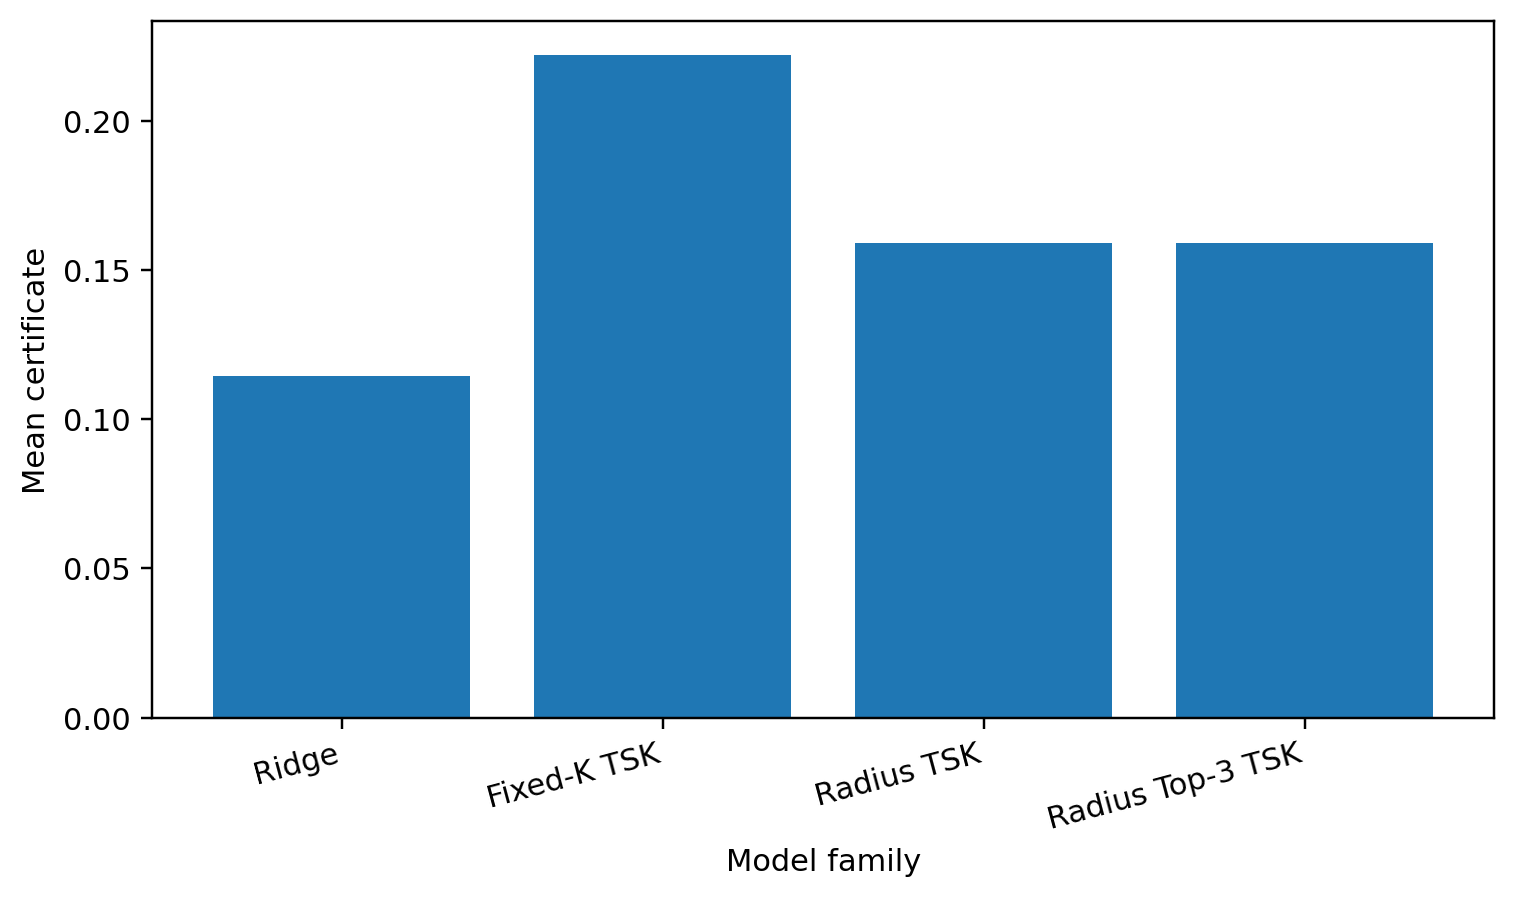
\includegraphics[width=\columnwidth]{figures/structural_certificate_by_family.png}
\caption{Mean familywise certificate under validation-RMSE selection across 30 synthetic development series. Ridge is tightest; radius control substantially improves on the originally prespecified fixed $K=12$ TSK baseline.}
\label{fig:structural_cert}
\end{figure}


\subsection{Fixed-$K$ Sensitivity Qualifies the Radius Advantage}
\begin{table}[htbp]
\caption{Fixed-$K$ sensitivity under validation-RMSE selection across 30 synthetic development series. The paired difference is Radius TSK minus Fixed-$K$ TSK; negative values favor radius control.}
\label{tab:fixed_k_sensitivity}
\centering
\footnotesize
\begin{tabular}{rrrrrr}
\toprule
$K$ & Dimension & Gaussian KL & Certificate & Test RMSE & $\Delta$ Cert. \\
\midrule
2 & 23.7 & 10.180 & 0.1326 & 0.8850 & +0.0264 \\
3 & 34.3 & 13.469 & 0.1465 & 0.8846 & +0.0125 \\
4 & 41.9 & 17.294 & 0.1568 & 0.8869 & +0.0021 \\
6 & 60.0 & 21.011 & 0.1701 & 0.8950 & -0.0112 \\
8 & 82.9 & 26.413 & 0.1875 & 0.8951 & -0.0286 \\
12 & 135.6 & 39.547 & 0.2221 & 0.9149 & -0.0631 \\
\bottomrule
\end{tabular}
\end{table}


Table~\ref{tab:fixed_k_sensitivity} shows that the mean fixed-$K$ certificate increases steadily with rule count, from 0.1326 at $K=2$ to 0.2221 at $K=12$. The radius-controlled mean is 0.1589. Consequently, radius control is not uniformly tighter than fixed rule bases: its mean certificate is looser than fixed $K=2$ and $K=3$, essentially matched by $K=4$, and tighter than the larger $K=6,8,12$ alternatives. After Holm correction, the paired certificate advantage is clear for $K=8$ and $K=12$, while the differences for $K=3,4,6$ are not statistically decisive.

When each series is allowed to choose its best fixed $K$ by validation RMSE, radius control changes the certificate by only $-0.0068$ on average (radius minus best fixed $K$; 95\% bootstrap interval $[-0.0190,0.0047]$; Holm-adjusted $p=0.382$). The corresponding test-RMSE mean difference is $-0.0054$ with bootstrap interval $[-0.0116,-0.0003]$, whereas the corrected rank test remains non-significant ($p=0.285$). The differing conclusions reflect that the bootstrap targets the mean while the signed-rank test targets the paired rank distribution and is affected by ties and heterogeneous effects. Nine of 30 series select $K=2$, five select $K=3$, four select $K=4$, six select $K=6$, five select $K=8$, and only one selects $K=12$. Under certificate selection, all 30 series select fixed $K=2$.

These results materially narrow the structural claim. Radius construction is useful as an adaptive mechanism that avoids large unnecessary rule bases, but the certificate gain relative to $K=12$ is mainly a rule-count effect. The current evidence does not show that radius control dominates a predeclared and fairly charged small fixed-$K$ grid.

\begin{figure}[htbp]
\centering
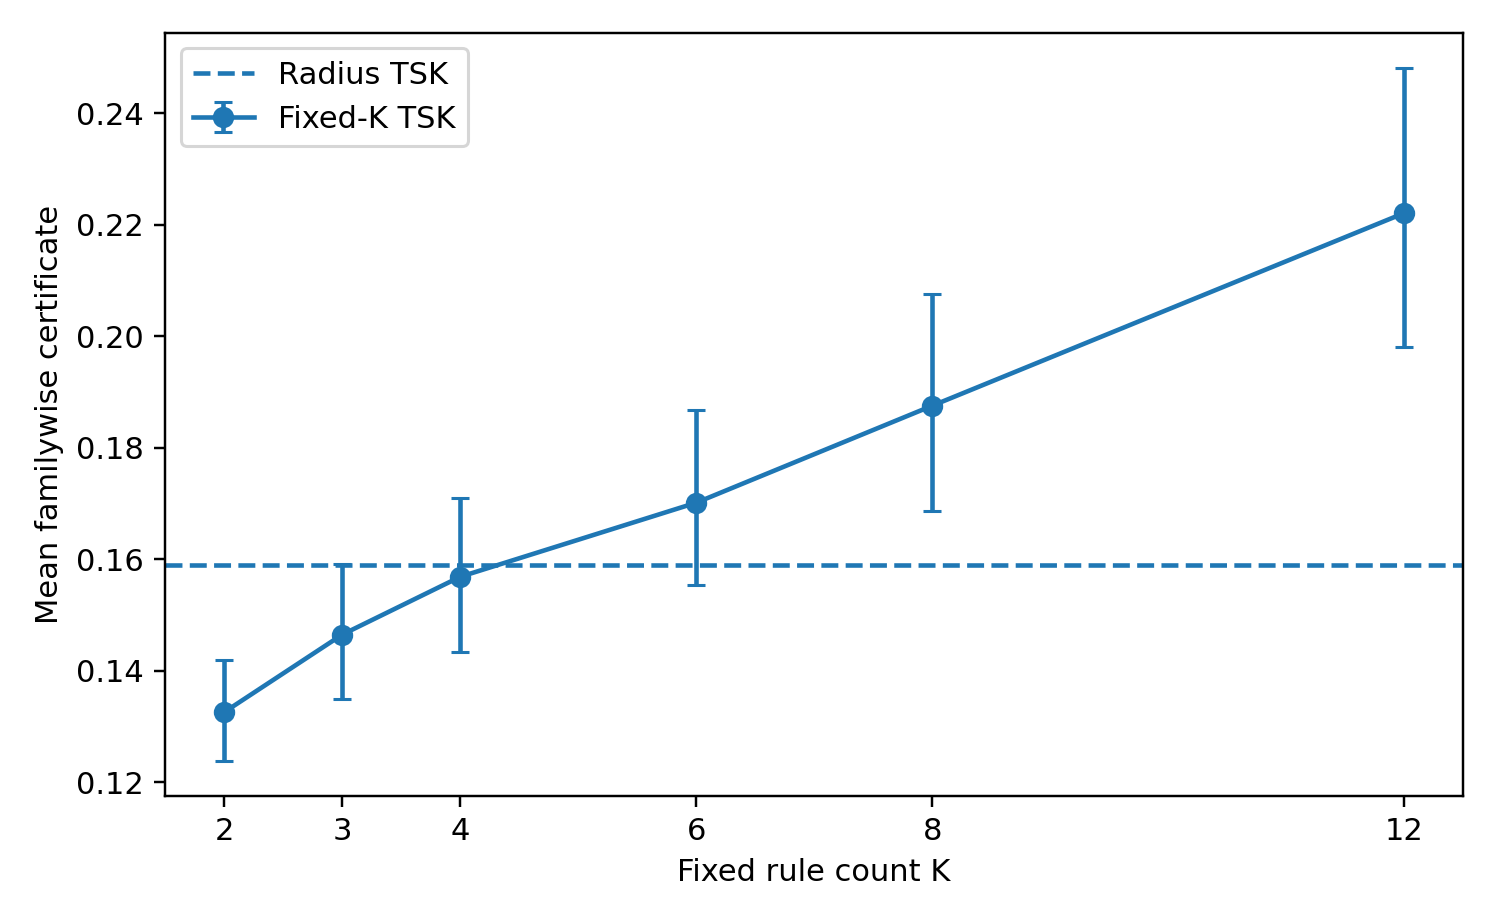
\includegraphics[width=\columnwidth]{figures/fixed_k_certificate_sensitivity.png}
\caption{Mean familywise certificate for fixed-$K$ TSK under validation-RMSE selection. Error bars are bootstrap intervals for the per-series means; the dashed line is the radius-controlled TSK mean.}
\label{fig:fixed_k_sensitivity}
\end{figure}

\begin{figure}[htbp]
\centering
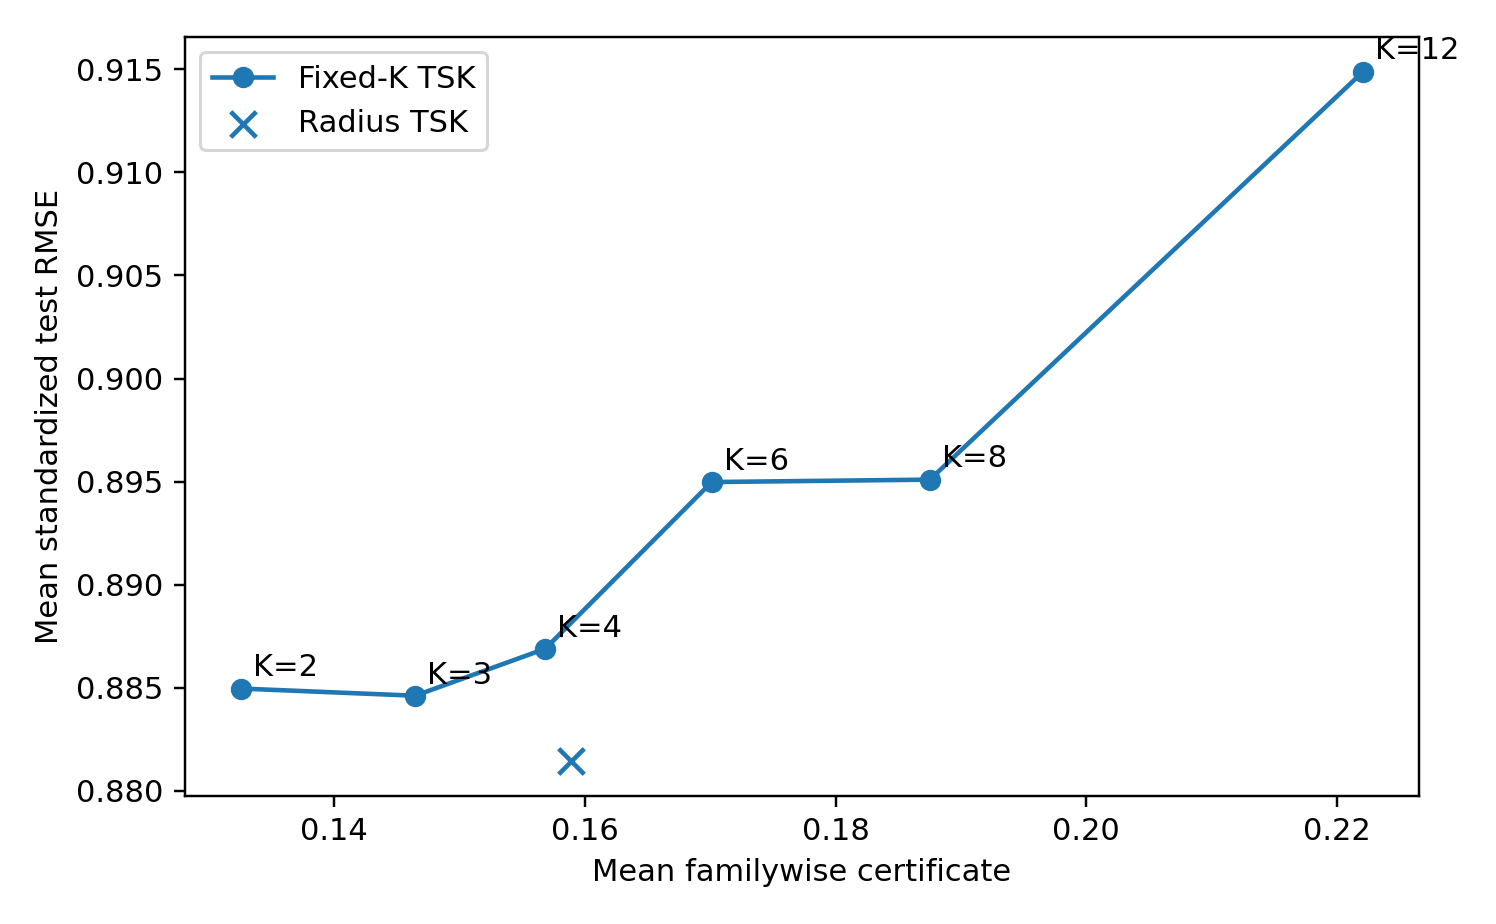
\includegraphics[width=\columnwidth]{figures/fixed_k_pareto_sensitivity.png}
\caption{Development mean test RMSE versus mean familywise certificate across fixed rule counts and radius-controlled TSK. The plot is descriptive and does not imply a universal Pareto ordering.}
\label{fig:fixed_k_pareto}
\end{figure}

\subsection{The Radius--Rule--Dimension--KL Chain}
Within each process, family, and lag, Spearman correlations across radius values average $-0.847$ for radius versus rule count, $1.000$ for rule count versus dimension, $0.981$ for dimension versus Gaussian KL, and $0.982$ for Gaussian KL versus certificate. These are descriptive associations rather than a universal monotonicity theorem, but they make the realized complexity path observable:
\begin{equation}
r\longrightarrow K(r)\longrightarrow D(r)\longrightarrow \mathrm{KL}\longrightarrow \operatorname{Cert}.
\end{equation}

Ridge retains the smallest mean certificate under both selection strategies: 0.1145 under validation-RMSE selection and 0.1017 under certificate selection. Under validation-RMSE selection, Radius TSK exceeds ridge by 0.0445 in certificate value (95\% CI $[0.0296,0.0609]$; Holm-adjusted $p<10^{-8}$), while its mean test-RMSE difference is small and uncertain ($-0.0052$, 95\% CI $[-0.0194,0.0137]$). The results therefore do not support a claim that TSK is intrinsically easier to certify than a linear model.

\subsection{Predictive Accuracy and Clipping}
\begin{table}[htbp]
\centering
\caption{Synthetic development results selected by validation RMSE (five seeds per process). RMSE is on the prior-standardized scale.}
\label{tab:process_results}
\small
\setlength{\tabcolsep}{5pt}
\begin{tabular}{lrrrrrr}
\toprule
& \multicolumn{2}{c}{Test RMSE} & \multicolumn{2}{c}{Certificate} & \multicolumn{2}{c}{Target clipping} \\
\cmidrule(lr){2-3}\cmidrule(lr){4-5}\cmidrule(lr){6-7}
Process & Ridge & Radius TSK & Ridge & Radius TSK & Cert. & Test \\
\midrule
AR(2) & 0.9098 & 0.9126 & 0.1128 & 0.1271 & 0.62\% & 0.35\% \\
SETAR & 1.0140 & 0.9798 & 0.1131 & 0.1467 & 0.42\% & 0.50\% \\
NARMA-10 & 0.7670 & 0.7656 & 0.1093 & 0.1188 & 0.97\% & 0.30\% \\
Mackey--Glass & 0.0656 & 0.0539 & 0.1129 & 0.2403 & 0.92\% & 1.30\% \\
GARCH & 1.0398 & 1.0926 & 0.0941 & 0.1114 & 0.25\% & 0.20\% \\
Structural break & 1.5236 & 1.4841 & 0.1445 & 0.2093 & 23.87\% & 71.55\% \\
\bottomrule
\end{tabular}
\end{table}


Table~\ref{tab:process_results} separates predictive accuracy from certificate tightness. Radius TSK improves mean test RMSE over ridge on SETAR, NARMA-10, Mackey--Glass, and the structural-break process, but is slightly worse on AR(2) and materially worse on GARCH. Its largest benefit is Mackey--Glass, where mean RMSE falls from 0.0656 to 0.0539, while its certificate is more than twice the ridge value because of additional complexity.

The structural-break process is a failure-boundary example. Certification target clipping is 23.87\% and test target clipping is 71.55\%. The bounded certificate remains formally meaningful for the clipped loss, but it is not an operational description of raw errors after the break.

The localized prior improves the selected familywise certificate over a zero-mean prior in 85.6\% of selected rows, with mean absolute improvement 0.0138 after charging the same prior-variant mixture cost. Localization is useful but not uniformly superior; GARCH contains counterexamples.

\subsection{Actual Multi-Rule Fuzzy Structures}
\begin{table}[htbp]
\centering
\caption{
Examples of actual multi-rule posterior-center TSK models.
Antecedent prototypes and consequent coefficients are reported in original data
units. Mean firing is computed over bound and validation observations.
The listed rules provide structural audit examples; PAC-Bayes guarantees apply
to the Gibbs predictor and clipped Bayesian model average rather than these
deterministic point predictors.
}
\label{tab:fuzzy_rule_examples}
\scriptsize
\renewcommand{\arraystretch}{1.12}
\setlength{\tabcolsep}{2.5pt}
\begin{tabularx}{\linewidth}{
  >{\RaggedRight\arraybackslash}p{1.55cm}
  >{\centering\arraybackslash}p{0.45cm}
  >{\centering\arraybackslash}p{0.72cm}
  >{\centering\arraybackslash}p{0.85cm}
  >{\raggedleft\arraybackslash}p{1.25cm}
  >{\raggedleft\arraybackslash}p{1.25cm}
  >{\RaggedRight\arraybackslash}X
}
\toprule
Example &
Rule &
\shortstack{Prior\\support} &
\shortstack{Mean\\firing} &
\shortstack{Center\\mean} &
\shortstack{Recent--\\oldest} &
Dominant local consequent terms \\
\midrule
SETAR seed 3001 & R1 & 143 & 34.1\% & -0.11 & 0.04 &
$+0.458y(t-1)+0.179y(t-2)+0.119y(t-3)$ \\
SETAR seed 3001 & R4 & 74 & 19.0\% & 0.06 & 0.24 &
$+0.487y(t-2)-0.422y(t-1)-0.037y(t-3)$ \\
SETAR seed 3001 & R3 & 82 & 18.5\% & -0.37 & 0.09 &
$+0.685y(t-1)+0.067y(t-2)-0.006y(t-3)$ \\
SETAR seed 3001 & R5 & 61 & 15.3\% & -0.01 & -0.23 &
$+0.183y(t-1)+0.106y(t-3)+0.003y(t-2)$ \\
SETAR seed 3001 & R2 & 37 & 13.1\% & -0.19 & -0.56 &
$+0.576y(t-1)-0.160y(t-3)+0.067y(t-2)$ \\
\midrule
Tetouan Zone 1 & R1 & 216 & 25.5\% & 31094.05 & 5904.95 &
$+0.641y(t-12)+0.463y(t-1)+0.259y(t-6)$ \\
Tetouan Zone 1 & R2 & 216 & 25.0\% & 31033.57 & -2317.05 &
$+0.927y(t-1)-0.198y(t-2)+0.164y(t-7)$ \\
Tetouan Zone 1 & R4 & 216 & 24.9\% & 31018.71 & -1208.12 &
$+0.888y(t-1)+0.459y(t-12)-0.299y(t-4)$ \\
Tetouan Zone 1 & R3 & 214 & 24.5\% & 30957.31 & -3487.66 &
$+0.542y(t-12)-0.466y(t-10)+0.356y(t-2)$ \\
\bottomrule
\end{tabularx}
\end{table}

The labels ``SETAR seed 3001'' and ``Tetouan Zone 1'' identify specific fitted diagnostic examples; they are not linguistic rule names or externally validated physical regimes.
Table~\ref{tab:fuzzy_rule_examples} reports two reconstructed posterior-center TSK models in original units. The five SETAR rules partition different lag configurations and attach distinct local affine dynamics; for example, the dominant rule places most weight on $y_{t-1}$, while another assigns a negative coefficient to $y_{t-1}$ and a larger positive coefficient to $y_{t-2}$. The four Tetouan rules have similar average load levels but different recent-versus-oldest prototypes and different combinations of the most recent, six-step, and twelve-step lags. This demonstrates that the implementation contains genuine local rule variation rather than repeated copies of one global affine model.

The interpretation must remain limited. These prototypes are data-driven summaries, not linguistic rules validated by domain experts. The Tetouan model also failed operationally on the held-out horizon, so interpretability does not imply predictive reliability. Full centers, spreads, local intercepts, all lag coefficients, supports, and firing frequencies are provided in the supplementary CSV artifact.

\subsection{Negative Tetouan Development Outcome}
The initial Tetouan gate admits a radius TSK model in zone 1 and a fixed-$K$ TSK model in zone 2, while zone 3 abstains. Both learned deployments fail on the test horizon: RMSE changes are $-11.86\%$ and $-1.51\%$, and asymmetric-cost changes are $-22.67\%$ and $-19.05\%$. With seven-day moving blocks, the zone-1 RMSE interval is $[-24.45,-1.04]\%$ and its cost interval is $[-34.95,-10.98]\%$; zone 2 has RMSE interval $[-13.04,8.55]\%$ and cost interval $[-35.35,-3.70]\%$. Zone 3 is identically the fallback. Averaged over all three zones, RMSE worsens by 4.46\% and cost worsens by 13.91\%.

This negative result demonstrates that a non-vacuous certificate plus overall validation performance is not a sufficient deployment rule under temporal shift. It motivated the stricter margin and block-stability requirements in the later internally locked PJM holdout protocol.

\subsection{Independent Internally Locked PJM Holdout Outcome}
\begin{table}[htbp]
\centering
\caption{
Frozen deployment decisions produced by the proposed auditable forecasting
framework. Improvements are reported relative to the predeclared seasonal-naive
fallback; negative values indicate degradation.
}
\label{tab:energy_decisions}
\footnotesize
\renewcommand{\arraystretch}{1.15}
\setlength{\tabcolsep}{2.5pt}
\begin{tabularx}{\linewidth}{
  >{\RaggedRight\arraybackslash}p{2.15cm}
  >{\RaggedRight\arraybackslash}X
  >{\centering\arraybackslash}p{1.35cm}
  >{\centering\arraybackslash}p{1.55cm}
  >{\centering\arraybackslash}p{1.55cm}
}
\toprule
Case &
Deployment &
Cert. &
\parbox[c]{1.55cm}{\centering Test RMSE\\improvement} &
\parbox[c]{1.55cm}{\centering Test cost\\improvement} \\
\midrule
Tetouan Zone 1 & Radius-controlled TSK & 0.1226 & -11.86\% & -22.67\% \\
Tetouan Zone 2 & Fixed-$K$ TSK & 0.1482 & -1.51\% & -19.05\% \\
Tetouan Zone 3 & Seasonal naive & -- & 0.00\% & 0.00\% \\
\midrule
PJM holdout -- AEP & Ridge & 0.0959 & 57.97\% & 58.64\% \\
PJM holdout -- COMED & Ridge & 0.0841 & 55.40\% & 54.11\% \\
PJM holdout -- DAYTON & Radius-controlled TSK & 0.0933 & 49.13\% & 50.30\% \\
PJM holdout -- PJME & Ridge & 0.0959 & 51.70\% & 51.42\% \\
\bottomrule
\end{tabularx}
\end{table}

\begin{table}[htbp]
\centering
\caption{Secondary paired moving-block-bootstrap uncertainty intervals for the frozen PJM test improvements. Circular blocks of 14 days and 20,000 resamples are used; 7- and 28-day sensitivity results are provided in the artifact. The analysis was added after the frozen test outcomes and does not alter the decisions.}
\label{tab:pjm_bootstrap_ci}
\footnotesize
\setlength{\tabcolsep}{3pt}
\begin{tabular}{lll}
\toprule
Region & RMSE improvement [95\% CI] & Cost improvement [95\% CI] \\
\midrule
AEP & 57.97\% [53.06, 61.61] & 58.64\% [54.00, 62.43] \\
COMED & 55.40\% [49.58, 59.83] & 54.11\% [48.31, 58.81] \\
DAYTON & 49.13\% [43.81, 53.53] & 50.30\% [45.16, 54.74] \\
PJME & 51.70\% [45.80, 56.29] & 51.42\% [45.71, 56.34] \\
\bottomrule
\end{tabular}
\end{table}


The frozen PJM gate admits a learned model in all four regions. Test RMSE improves by 57.97\%, 55.40\%, 49.13\%, and 51.70\% for AEP, COMED, DAYTON, and PJME, respectively. Corresponding asymmetric-cost improvements are 58.64\%, 54.11\%, 50.30\%, and 51.42\%; mean improvements are 53.55\% and 53.62\%. Table~\ref{tab:pjm_bootstrap_ci} reports secondary 14-day moving-block-bootstrap intervals. Every lower bound remains positive, and the same conclusion holds under 7- and 28-day block-length sensitivity analyses. Selected certificates range from 0.0841 to 0.0959, and test target and forecast clipping are zero.

\begin{figure}[htbp]
\centering
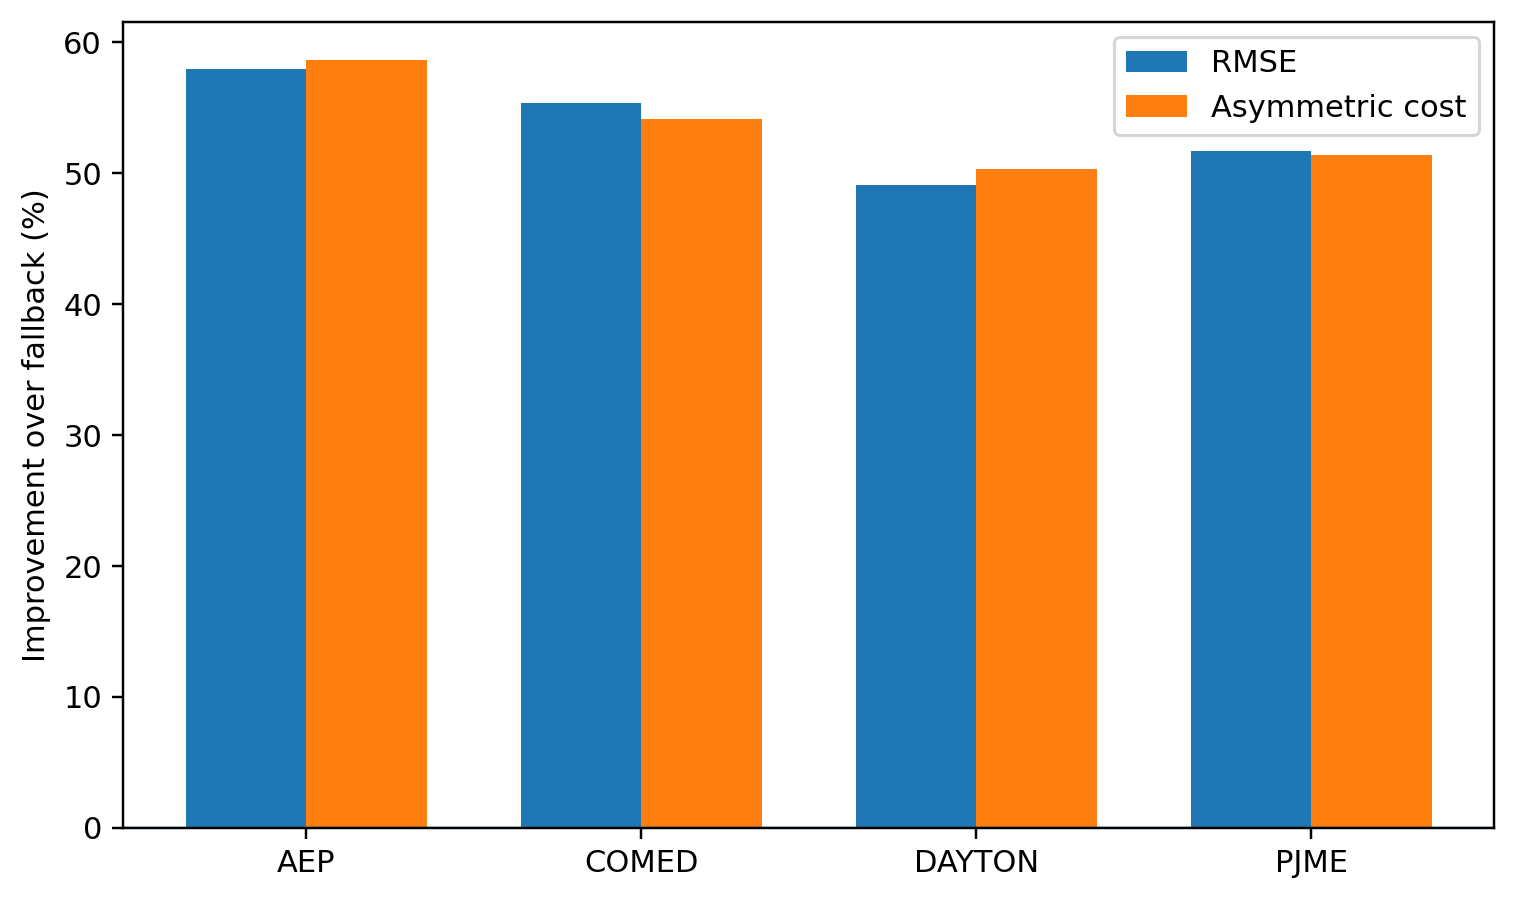
\includegraphics[width=\columnwidth]{figures/pjm_test_improvements.png}
\caption{Independent PJM test improvements over the frozen seven-day seasonal-naive fallback.}
\label{fig:pjm_improvements}
\end{figure}

The internally locked PJM holdout result does not establish nonlinear fuzzy superiority. AEP, COMED, and PJME select ridge. DAYTON selects a radius-controlled one-rule TSK with lag 14; with one rule, this is an affine predictor. No fixed-eight-rule TSK candidate passes the frozen gate. The operational evidence therefore supports a complexity-aware gate that can shrink to a simple model, not a claim that a multi-rule TSK system caused the gain.

\subsection{Retrospective Exact-BMA Alignment Audit}
\begin{table*}[htbp]
\centering
\caption{Strictly retrospective exact-clipped-BMA alignment audit of the
frozen selected energy candidates. Candidate identities are preserved. The
original seven-condition gate and thresholds are preserved for PJM and
transferred to Tetouan only as a post-hoc abstention diagnostic;
posterior-scale selection and gate evaluation exclude test outcomes. Positive changes indicate improvement over the predeclared seasonal
fallback. ``Score'' denotes the two-to-one asymmetric forecasting-error
score, not a monetized economic cost.}
\label{tab:retrospective_bma_alignment}
\scriptsize
\setlength{\tabcolsep}{4pt}
\begin{tabular}{llrrrrrr}
\toprule
Case & Series & Exact cert. & Gate &
Val. RMSE & Val. score & Test RMSE & Test score \\
\midrule
Tetouan & Zone 1 & 0.1196 & Fail & 20.19\% & 16.63\% & -9.07\% & -21.22\% \\
Tetouan & Zone 2 & 0.1368 & Fail & 35.19\% & 35.65\% & -25.70\% & -65.03\% \\
\midrule
PJM & AEP    & 0.0953 & Pass & 53.11\% & 54.58\% & 57.96\% & 58.63\% \\
PJM & COMED  & 0.0839 & Pass & 46.95\% & 49.54\% & 55.45\% & 54.11\% \\
PJM & DAYTON & 0.0929 & Pass & 45.60\% & 46.29\% & 49.14\% & 50.21\% \\
PJM & PJME   & 0.0958 & Pass & 53.86\% & 52.96\% & 51.71\% & 51.42\% \\
\bottomrule
\end{tabular}
\end{table*}


Table~\ref{tab:retrospective_bma_alignment} reports the strictly retrospective
alignment audit. The two frozen Tetouan deployments are rejected by the
stricter exact-BMA gate. Zone 1 fails both the exact certificate threshold and
the worst-block degradation condition; zone 2 fails the exact certificate
threshold alone. Exact-BMA test performance is worse than the seasonal fallback in both
zones. The post-hoc transfer of the PJM gate rejects both candidates,
showing only that this later rule would have abstained; it does not show
that the original Tetouan protocol would have done so. This is a post-hoc
diagnostic of abstention value, not a causal, prospective, or internally
locked estimate. Tetouan zone 3 is not
listed because its frozen deployment is already the fallback and has no
selected posterior.

All four frozen PJM selections pass every exact-BMA gate condition. Each has
nonnegative improvement in all four validation blocks and a positive
worst-block margin. Their exact-BMA test improvements over the seven-day
seasonal fallback remain approximately $49$--$58\%$ in RMSE and
$50$--$59\%$ in the asymmetric forecasting-error score. Relative to the
original posterior-center forecasts, exact BMA changes PJM RMSE by less than
$0.11\%$ in magnitude. Its value here is therefore theoretical and
operational alignment, not an additional accuracy claim. Because the audit
was designed after the original outcomes were opened, it cannot strengthen
the original internally locked interpretation.

\subsection{Secondary Post-Hoc Statistical Benchmarks}
The post-hoc SARIMA and ETS comparisons provide a stricter context for the PJM result. Across the four regions, selected SARIMA specifications improve RMSE over the seasonal-naive fallback by 56.82\% on average and improve on the originally deployed point forecasts by 6.99\%. ETS improves over the fallback by 54.77\% on average and over the deployed forecasts by 2.43\%. SARIMA has lower test RMSE than the deployed model in all four regions; ETS is better in AEP and DAYTON, essentially tied in COMED, and worse in PJME. The full per-region table is reported in the supplementary material.

These comparisons were designed after the original PJM outcomes were opened. They therefore cannot be used to revise the frozen gate or strengthen the original internally locked claim. Instead, they show that the large gain over seasonal naive is not unique to the PAC-Bayesian candidate family and that simple statistical forecasting models remain competitive or superior. The operational contribution is consequently the auditable screening and abstention protocol, not state-of-the-art point forecasting.

	\section{Discussion and Limitations}
\label{sec:discussion}

\subsection{An Integration Result, Not a Model-Superiority Result}
The strongest contribution of the study is methodological integration. The framework places chronological prior construction, complete structural coding, Gaussian posterior localization, bounded sequential risk, model selection, and operational abstention inside one auditable pipeline. Each element is individually established or technically standard; the contribution lies in making their interaction explicit and reproducible for linear and TSK forecasters under temporal dependence.

The structural experiments support a precise but limited mechanism. Replacing an unnecessarily dense 12-rule TSK model with a smaller rule base reduces randomized dimension, Gaussian KL, and certificate value. The Fixed-$K$ sensitivity analysis shows, however, that small predeclared fixed rule bases can match or improve on radius control. The supported conclusion is therefore that removal of complete rule blocks matters for the charged complexity. The present evidence does not establish that radius construction is intrinsically superior to every alternative way of choosing a compact rule base.

Top-3 activation provides a complementary negative result. It changes the number of rules evaluated at a sample but leaves the randomized consequent dimension unchanged. Its negligible certificate effect is therefore consistent with the mathematical accounting. For certificate-aware fuzzy design, sparsity must operate on the parameterized rule structure or on a posterior over rule inclusion, not only on firing-strength truncation at prediction time.

\subsection{Interpretability and Its Boundary}
The reconstructed SETAR and Tetouan rules show that the implementation learns distinct local affine relationships associated with different antecedent prototypes. This is useful for auditing the model and checking that a multi-rule TSK system is not merely duplicating one global regression. It is not evidence that the prototypes correspond to physically validated regimes, and it is not evidence that interpretability guarantees robustness. The Tetouan multi-rule model is the clearest warning: its rules are inspectable, yet the deployment decision fails on the held-out horizon.

The original operational forecasts are deterministic posterior-center
predictions, whereas the PAC-Bayesian guarantee directly covers the Gibbs
predictor and, by convexity, the clipped Bayesian model average. Before
clipping, the posterior mean of a linear-in-consequents TSK predictor equals
the posterior-center prediction. After clipping, equality with the clipped
BMA generally fails. The frozen V3 results must therefore remain described as
posterior-center results.

The retrospective V5 audit evaluates this prediction-object mismatch only at
the diagnostic level. With exact clipped BMA and exact empirical Gibbs risk, all four frozen PJM
selections still satisfy their unchanged PJM gate. A post-hoc transfer of
that gate rejects the two frozen Tetouan deployments; this does not
establish what the original Tetouan gate would have decided. This pattern is consistent with the intended role
of screening and abstention, but it is not a new prospective or internally locked result because
the alignment audit was specified after both outcome sets were available. A
prospective replication must make exact clipped BMA the operational forecast
from the outset.

\subsection{Operational Evidence and Stronger Baselines}
The negative Tetouan study and positive internally locked PJM holdout illustrate why a certificate alone is not a deployment rule. The redesigned PJM gate combines certificate thresholding with validation margins and blockwise temporal-stability checks. Moving-block-bootstrap intervals remain positive for the original PJM comparison with seasonal naive, but these intervals quantify uncertainty only for the observed trajectories and do not prove population-level transfer to other regions or future regimes.

The secondary SARIMA and ETS analysis materially narrows the operational interpretation. SARIMA improves on the originally deployed point forecast in all four PJM regions, while ETS is competitive and sometimes better. Because these comparisons were designed after the PJM outcomes were opened, they are post hoc and cannot replace the frozen protocol. They nevertheless show that the gain over seasonal naive is not specific to TSK or PAC-Bayesian selection. The defensible operational contribution is an auditable process for screening, margin checking, and abstention, not superior forecasting accuracy relative to established statistical methods.

\subsection{Limits of the Certificate}
The certificate controls average conditional risk of a clipped Gibbs predictor over the certification horizon and transfers to the clipped BMA. It does not control raw RMSE, the deterministic posterior-center predictor, an unseen future horizon, or relative performance against another forecasting method. Structural-break experiments demonstrate the practical cost of the bounded-loss construction: when a prior-fixed clipping interval is exceeded frequently, the certificate remains formally valid for the clipped loss but loses relevance to raw-scale errors.

Heavy-tail or variance-adaptive supermartingale bounds \cite{haddouche2023heavy,rodriguez2024more} are a principled next step, but they require a separately verified implementation. The time-uniform proposition is evaluated numerically only at the final certification horizon; the paper does not claim an executed confidence sequence over all prefixes.

\subsection{Remaining Empirical and Procedural Limitations}
The synthetic study uses five seeds per process. The paired analysis is adequate for large structural contrasts such as Radius TSK versus fixed $K=12$, but it is not sufficient to characterize all nonlinear regimes or small performance differences. The PJM case contains four regional series over one common historical interval and uses no exogenous variables. The post-hoc statistical grid is intentionally simple and does not cover gradient boosting, modern probabilistic forecasting, or deep sequence models.

The PJM protocol is internally locked and supported by hashes, manifests, and pretest decision files, but it was not externally preregistered. A compute-only interruption occurred before test opening; recovery used unchanged locked inputs. The complete chronology is retained in the supplementary audit. These controls improve traceability but are not equivalent to an external timestamped preregistration.

\subsection{Implications for Future Fuzzy-System Research}
A stronger fuzzy contribution would replace deterministic radius construction with a posterior over rule inclusion or a certificate-aware structural learning objective. Such a method could jointly trade predictive fit, interpretable rule blocks, and charged complexity. It should be compared fairly with small fixed-$K$ grids and with strong statistical and machine-learning baselines. Domain-expert validation of learned rule semantics would also be needed before presenting local prototypes as operational explanations rather than model diagnostics.

	\section{Conclusion}
\label{sec:conclusion}

This work presents an auditable framework that combines chronological prior construction, explicit structural coding, a computable sequential PAC-Bayesian certificate, linear and TSK forecasting families, and conservative deployment screening. The general supermartingale inequality is established in prior work; the contribution is its fully charged, reproducible specialization and the empirical separation of different kinds of sparsity.

The structural experiments show that removing complete TSK rule blocks can reduce randomized dimension, Gaussian KL, and certificate value relative to an unnecessarily dense rule base. The additional Fixed-$K$ sensitivity prevents a stronger claim: small fixed rule bases can match or tighten the radius-controlled certificate, so the evidence supports structural compactness rather than universal superiority of radius selection. Sparse activation alone does not deliver the same complexity reduction when all consequent coordinates remain randomized and charged.

The energy studies show that a valid certificate can contribute to a broader
screening rule but cannot replace forecasting validation. The original
Tetouan gate fails. The redesigned PJM gate succeeds relative to its
predeclared seasonal-naive fallback, yet the selected models are linear or
one-rule affine predictors. A strictly retrospective exact-BMA alignment
audit rejects the two failed Tetouan selections and preserves acceptance of
all four frozen PJM selections, thereby addressing the certified-versus-
operational prediction mismatch diagnostically but not prospectively. For
Tetouan, the stricter gate is a post-hoc transfer rather than the original
frozen gate.
Secondary post-hoc SARIMA and ETS benchmarks often improve further on the
original deployed point forecasts. Accordingly, the real-data evidence
supports transparent model screening, validation margins, temporal-stability
checks, prediction-object alignment, and abstention; it does not establish
nonlinear fuzzy-model dominance or state-of-the-art forecasting accuracy.

The main conclusion is therefore modest: PAC-Bayesian complexity can be made
explicit and auditable for linear and TSK time-series models, and true
structural rule reduction can tighten that accounting. The present
implementation can evaluate exact clipped Gaussian BMA and exact expected
clipped loss, but the associated energy audit is retrospective. Future work
should deploy that prediction object prospectively under an externally
timestamped protocol, learn a posterior over rule inclusion, compare against
stronger forecasting baselines, and replace clipping with verified
heavy-tail or variance-adaptive sequential guarantees.

A particularly important direction is to develop a certificate-aware structural learning objective that jointly optimizes predictive fit and the PAC-Bayesian complexity term, rather than selecting rule structures through externally specified
radius or fixed-$K$ heuristics.


\section*{Data and Code Availability}

The source code, processed data, experimental configurations,
result tables, audit manifests, and supplementary materials
supporting this study are publicly available at
\url{https://github.com/muneeff/pacbayes-sparse-tsk}.

The exact version associated with this manuscript is archived as
release v4.3.1:
\url{https://github.com/muneeff/pacbayes-sparse-tsk/releases/tag/v4.3.1}.

Raw third-party datasets are not redistributed. Download,
verification, and preprocessing scripts are provided in the
repository.


\section*{CRediT Author Statement}
Muneef Abdulkareem Farea Ahmed: Conceptualization,
Methodology, Software, Validation, Formal analysis,
Investigation, Data curation, Visualization, Writing--original
draft, Writing--review and editing, and Project administration.

\section*{Funding}
This research did not receive any specific grant from funding
agencies in the public, commercial, or not-for-profit sectors.

\section*{Declaration of Competing Interest}
The author declares that he has no known competing financial
interests or personal relationships that could have appeared to
influence the work reported in this paper.

\section*{Declaration of Generative AI and AI-Assisted
	Technologies in the Manuscript Preparation Process}

During the preparation of this manuscript, the author used OpenAI ChatGPT to assist with language refinement, structural editing, and the organization of software and reproducibility documentation. The author independently reviewed and verified the mathematical arguments, experimental procedures, code, results, references, and final manuscript, and takes full responsibility for the content of the work.
	
	% =========================================================
	% References
	% =========================================================
	\bibliographystyle{elsarticle-num}
	\bibliography{refs}
	
\end{document}